\chapter{}
\section{Coeficientes indeterminados - Método de superposición}
\dfn{}{\textbf{DEFINICI\'ON:} Método para resolver ecuaciones diferenciales lineales no-homogéneas de segundo orden con coeficientes constantes. Se identifica la forma de la solución particular correspondiente a la parte no-homogénea, y se reemplaza por la función desconocida $(y)$ en la parte homogénea para obtener las constantes.}

\subsection{Pasos}

\begin{enumerate}
\item Identificar la forma de la solución particular correspondiente a la parte no-homogénea $f(x)$.

\item Reemplazar la solución particular en la parte homogénea para obtener las constantes $y = f(x)$.

\item Sumar la solución particular (con constantes halladas) con la solución homogénea [FIN].
\end{enumerate}

\nt{\textbf{No hace falta} que la ecuación esté en la forma estándar.}

\subsection{Tabla de soluciones particulares}

% imagen de la tabla
\begin{figure}[h]
    \centering
    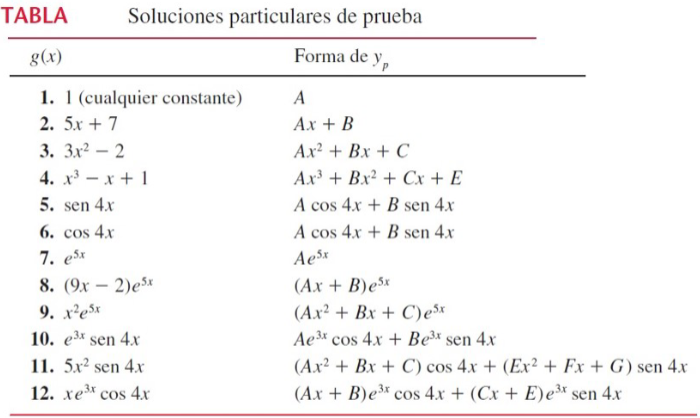
\includegraphics[width=0.8\textwidth]{tabla.png}
\end{figure}

\newpage

\subsection{Ejemplo combinado}
\ex{Resuelva la ecuación diferencial: $y''-9y'+14y=3x^2-5\sin2x+7xe^{6x}$}{
    Identificamos la forma de la solución particular correspondiente a la parte no-homogénea: 

    \[(Ax^2+Bx+C) + (D\cos 2x + E\sin 2x) + (Fx + G)e^{6x}\]

    Reemplazamos la solución particular en la parte homogénea para obtener las constantes:

    \[y = Ax^2+Bx+C + D\cos 2x + E\sin 2x + Fxe^{6x} + Ge^{6x}\]
    \[y' = 2Ax+B - 2D\sin 2x + 2E\cos 2x + 6Fxe^{6x} + 6Ge^{6x}\]
    \[y'' = 2A - 4D\cos 2x - 4E\sin 2x + 36Fxe^{6x} + 36Ge^{6x}\]

    *Reemplazando en la ecuación diferencial:*
    \begin{equation}
    \begin{split}
    & (2A - 4D\cos 2x - 4E\sin 2x + 36Fxe^{6x} + 36Ge^{6x}) \\
    -\; & 9(2Ax+B - 2D\sin 2x + 2E\cos 2x + 6Fxe^{6x} + 6Ge^{6x}) \\
    +\; & 14(Ax^2+Bx+C + D\cos 2x + E\sin 2x + Fxe^{6x} + Ge^{6x}) \\
    =\; & 3x^2-5\sin2x+7xe^{6x}
    \end{split}
    \end{equation}

    \begin{equation}
    \begin{split}
    & (2A - 4D\cos 2x - 4E\sin 2x + 36Fxe^{6x} + 36Ge^{6x}) \\
    +\; & (-18Ax - 9B + 18D\sin 2x - 18E\cos 2x - 54Fxe^{6x} - 54Ge^{6x}) \\
    +\; & (14Ax^2+14Bx+14C+14D\cos 2x+14E\sin 2x+14Fxe^{6x}+14Ge^{6x}) \\
    =\; & 3x^2-5\sin2x+7xe^{6x}
    \end{split}
    \end{equation}

    \begin{equation}
    \begin{split}
    & (14A)x^2 + (-18A + 14B)x + (2A - 9B + 14C) \\
    +\; & (10D-18E)\cos2x + (10E-18D)\sin2x \\
    +\; & (-4F)xe^{6x} + (-4G)xe^{6x} \\
    =\; & 3x^2-5\sin2x+7xe^{6x}
    \end{split}
    \end{equation}

    \begin{equation}
    \begin{split}
    & 14A = 3 \implies A = \frac{3}{14} \\
    & -18A + 14B = 0 \implies B = \frac{27}{98} \\
    & 2A - 9B + 14C = 0 \implies C = \frac{24}{98} \\
    & 10D-18E = 0 \implies D = \frac{9}{5}E \\
    & 10E-18D = -5 \implies E = \frac{25}{112} \land D = \frac{45}{112} \\
    & -4F = 7 \implies F = -\frac{7}{4} \\
    & -4G = 0 \implies G = 0
    \end{split}
    \end{equation}

    Finalmente, la solución particular es:
    \[
        y_P = \frac{3}{14}x^2 + \frac{27}{98}x + \frac{24}{98} + \frac{45}{112}\cos2x + \frac{25}{112}E\sin2x - \frac{7}{4}xe^{6x} 
    \]

}

\newpage

\nt{\textbf{Términos duplicados:} Si la parte no-homogénea tiene términos duplicados, se debe multiplicar la solución particular por $x$ hasta que no haya duplicados.}

\ex{Resuelva: $y'' - 2y' + y = e^x$}{
    En este caso no se puede usar $Ae^x$ como solución particular, ya que $c_1e^x$ es parte de la solución homogénea. Por lo tanto, multiplicamos por x.

    Observamos que tampoco se puede usar $Axe^x$, ya que $c_2xe^x$ es parte de la solución homogénea. Por lo tanto, multiplicamos otra vez por x.

    Finalmente, la solución particular es de forma $Ax^2e^x$, y no hay duplicados en la parte homogénea.

    Reemplazamos la solución particular en la parte homogénea para obtener las constantes:

    \[y = Ax^2e^x\]
    \[y' = 2Axe^x + Ax^2e^x\]
    \[y'' = 2Ae^x + 4Axe^x + Ax^2e^x\]

    *Reemplazando en la ecuación diferencial:*
    \begin{equation}
    \begin{split}
    & 2Ae^x + 4Axe^x + Ax^2e^x \\
    -\; & 2(2Axe^x + Ax^2e^x) \\
    +\; & (Ax^2e^x) \\
    =\; & e^x
    \end{split}
    \end{equation}

    \[2Ae^x = e^x\]
    \[A = \frac{1}{2}\]

    Finalmente, la solución particular es:
    \[y_P = \frac{1}{2}x^2e^x \]
}

